\documentclass[format=acmsmall, review=false, screen=true]{acmart}
\settopmatter{printacmref=false} % Removes citation information below abstract
\renewcommand\footnotetextcopyrightpermission[1]{} % removes footnote with conference information in first column
\pagestyle{plain} % removes running headers
\acmYear{2018}
\acmMonth{7}

\usepackage[utf8]{inputenc}
\usepackage{microtype}
\usepackage{amsmath}
\usepackage[procnames]{listings}
\usepackage{amsmath}
\usepackage{float}
\usepackage{wrapfig}
\usepackage{subcaption}
\usepackage{dirtytalk}
\usepackage{color}

\lstset{
  basicstyle=\ttfamily,
  columns=fullflexible,
  frame=single,
  breaklines=true,
  postbreak=\mbox{\textcolor{red}{$\hookrightarrow$}\space},
  aboveskip=10pt,
  belowskip=5pt,
  tabsize=2
}


\setlength{\textfloatsep}{15pt}
\setlength{\abovecaptionskip}{6pt}
\setlength{\belowcaptionskip}{6pt}

\author{Richard Banyi}
\affiliation{%
  \institution{IT University of Copenhagen}
  \streetaddress{Rued Langgaards Vej 7}
  \city{Copenhagen}
  \postcode{2300}
  \country{Denmark}
}

\email{riba@itu.dk}

\author{David Kadish}
\affiliation{%
  \institution{Supervisor}
}
\affiliation{%
  \institution{IT University of Copenhagen}
}
\affiliation{%
  \institution{Robotics, Evolution, and Art Lab}
}
\email{davk@itu.dk}

\author{Andres Faina}
\affiliation{%
  \institution{Supervisor}
}
\affiliation{%
  \institution{IT University of Copenhagen}
  \streetaddress{Rued Langgaards Vej 7}
  \city{Copenhagen}
  \postcode{2300}
  \country{Denmark}
}
\affiliation{%
  \institution{Robotics, Evolution, and Art Lab}
}
\email{anfv@itu.dk}


\title{\textsc{Thesis Preparation }}
\subtitle{\textsc{IT University of Copenhagen, Autumn 2018}}
\acmDOI{}
\begin{document}


\begin{abstract}
Donec euismod iaculis pretium. Donec non massa elit. Phasellus sagittis magna et maximus dictum. Duis quis ullamcorper orci. Mauris interdum, elit eu tincidunt tempor, lectus mi venenatis purus, quis posuere tellus ex in magna. Phasellus tincidunt nibh eu tortor semper, et varius justo vulputate. Nullam dictum congue lacinia. Maecenas sagittis nulla quis leo fringilla viverra. Proin eget egestas nisl. Class aptent taciti sociosqu ad litora torquent per conubia nostra, per inceptos himenaeos. Pellentesque habitant morbi tristique senectus et netus et malesuada fames ac turpis egestas. Vestibulum a interdum tellus, a hendrerit ligula. Duis ut risus ut lacus maximus euismod. Integer quis justo sit amet sapien accumsan rutrum nec nec dolor. Aliquam laoreet scelerisque ante, quis hendrerit ipsum viverra tempor.
\end{abstract}

\maketitle

\section{Introduction}

Intelligent agents are defined as entities that carry out some set of operations on behalf of a user 
or a program with some degree of independence or autonomy, and in so doing, employ some knowledge or 
representation of the user's goals or desires. \footnote{\url{https://en.wikipedia.org/wiki/Autonomous_agent}}

Unfinished...

\section{Related Work}

In the machine learning field, teaching agents to learn different behaviors, is generally refered to as \emph{multimodal behavior} \footnote{\url{http://nn.cs.utexas.edu/?li:alife14}}. For example an haversting robot will have to behave differently depending whether it is harvesting tomatos, strawberries \footnote{\url{http://www.dogtoothtech.com/}}, or searching for a dock to charage. Learning multimodal behaviors can be diffult to solve directly. Many papers suggest to decouple the complex task into smaller related tasks. Rather than learning the complex task at once they focus on learning smaller related task first. The tasks are than combined and adjusted to form a more complex task. Therefore the smaller tasks represents crucial \emph{stepping stones} towards solving the complete task. The challenge is how to properly decouple the complex task into many subtask and in which order these subtask should interlieve to effectively form a more sophisticated behavior.

Joost Huizinga and Jeff Clune gave a good example \ref{fig:jumping_running} how these challenges can emerge in robot training task, which has to be able to learn both to run and jump. In their hypothetical example their argue, that running is much easier to learn than jumping, but learning to jump well first is an important stepping stone in order to become excelend in both tasks. Therefore individuals who are better at running, are more favorable than individuals that are average at jumping, and those individuals who are good at jumping are not selected in the future generations. An important stepping stone is lost during evolution. 

\begin{figure}[H]
  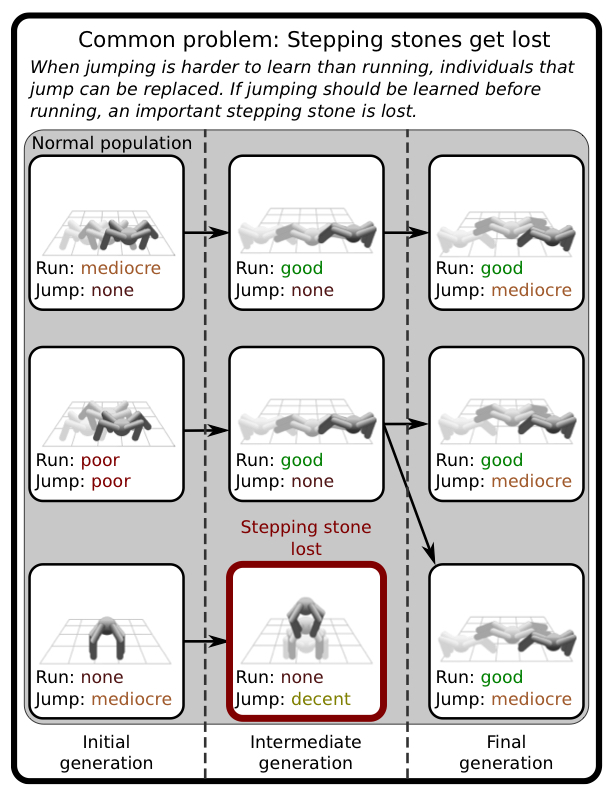
\includegraphics[width=0.46\linewidth]{img/jumping_running.JPEG}
  \caption{\label{fig:jumping_running}Stepping stones get lost}
\end{figure}

Joost Huizinga and Jeff Clune designed \emph{Combinatorial Multi-Objective Evolutionary Algorithm (CMOEA)} which is able to preserve the stepping stones of multimodal problems. The algorithm divides the population into bins, every bin is a combination of subtasks. Each set of subtasks has its own fitness function. The population is competing within bins, which helps to preserve important stepping stones to solve the overall problem. They have succesfully evolved a controller on a multimodal robotics problem with six subtaks.

The six tasks \emph{Forward, Backward, Turn-left, Turn-right, Jump, Crouch} needed to be learned by the robot. \emph{CMOEA} starts by generating a random number of individuals and adding copy of each individual to every bin. Selection is performed within each bin, with respect to the subtask associated with that bin. Each generation the algorithm selects a number of parents randomly across all bins. Each selected parents produce only one child by applying mutation (no crossver is applied) and is copied to every bin, afterwards selection is applied within each bin. The survivor selection method is applied by \emph{NSGA-II} with performance on the task associated with the given bin as one objective and \emph{behavioral diversity}\footnote{\url{https://www.researchgate.net/publication/51568478_Encouraging_Behavioral_Diversity_in_Evolutionary_Robotics_An_Empirical_Study}} as the other objective. Behavioral diversity ensure that individuals within each bin solves the same subtask in different ways. It's implemented by measuring the distance of some behavioral features between each individual in the same bin. All the controllers are neural networks evolved with \emph{NEAT} mutation operators without crossover, encoded with \emph{HyperNEAT}\footnote{\url{http://eplex.cs.ucf.edu/hyperNEATpage/}} encoding, which is extended with \emph{Multi-Spatial Substrate (MSS)}\footnote{\url{http://eplex.cs.ucf.edu/papers/pugh_gecco13_revised.pdf}} and a \emph{Link Expression Output}\footnote{\url{http://eplex.cs.ucf.edu/papers/verbancsics_gecco11.pdf}}.

\begin{figure}[H]
  \centering
  \begin{subfigure}[t]{0.55\textwidth}
    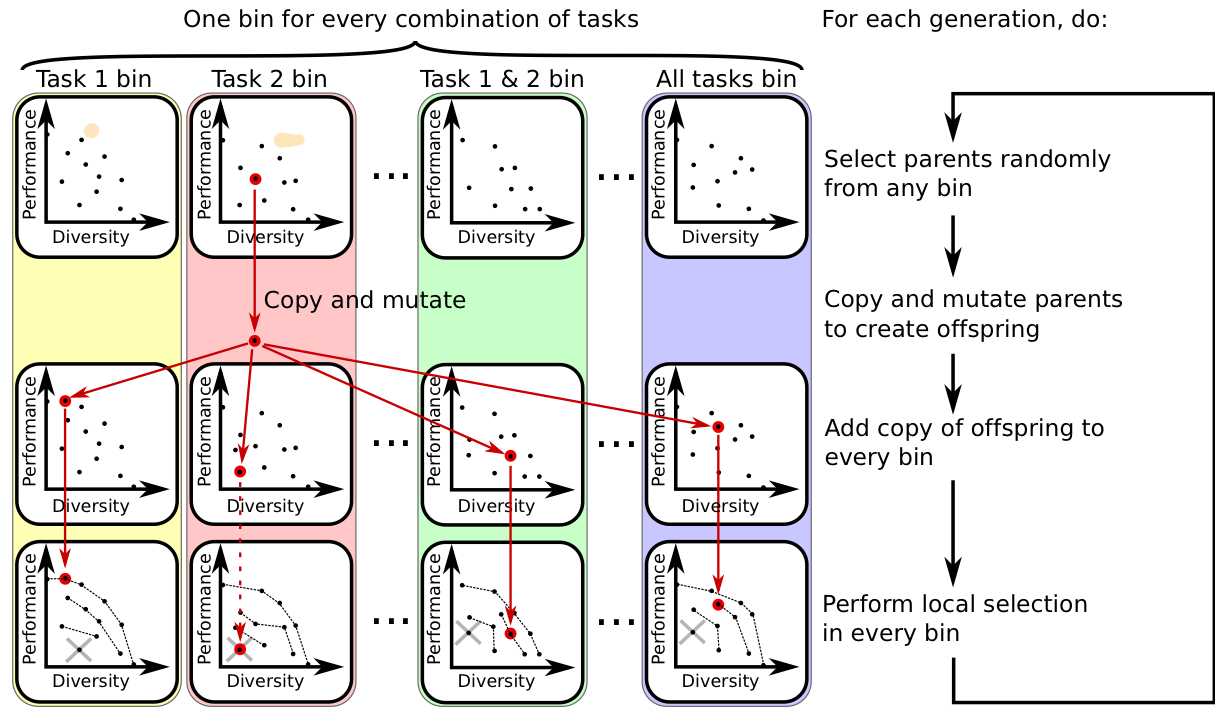
\includegraphics[width=\textwidth]{img/cmoea.JPEG}
    \caption{\label{fig:fronts}Overview of CMOEA}
  \end{subfigure}
  \hfill
  \begin{subfigure}[t]{0.43\textwidth}
    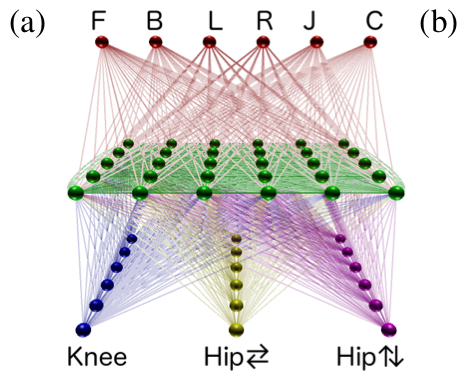
\includegraphics[width=\textwidth]{img/hyperneat.JPEG}
    \caption{\label{fig:endings}The spatial network layout, MSS planes.}
  \end{subfigure}
\end{figure}

\section{Algorithms}

\subsection{Evolutionary Algorithms}

\emph{Evolutionary algorithms} focus on global optimization problems inspired by biological evolution. EA are population based, meta heuristic search procedures that incorporate genetic operators. Algorithm maintains a population of candidate solutions which is subjected to natural selection and mutation \footnote{\url{https://en.wikipedia.org/wiki/Evolutionary_algorithm}}. In each generation, a set of offspring is generated by applying bio operators such as \emph{mutation, crossover, selection}. Each generation, the fitness of every individual in the population is evaluated. More fit individuals are stochastically selected from the current population, and each individual's \emph{genome} is modified (recombined or randomly mutated) to form a new generation. The algorithm terminates when either the maximum number of generations has been produced, or fitness level has been reached for the population.

\subsection{Non-Dominated Sorting Genetic Algoritm II}

Multi-objective optimization is concerned with optimization problems which involves several objective functions to be optimized simultaneously. For example an objective for a problem may require to minimize cost while maximazing profits, thus these two contradicting objectives can't be optimized simultaneously. Maximizing one objective leads to weakening the other objective. Therefore there is no single feasible solution, but instead a set of \emph{Pareto} optimal solutions.  A solution is called \emph{non-dominated}, if none of the objective functions can be improved in value without degrading some of the other objective values \footnote{\url{https://en.wikipedia.org/wiki/Multi-objective_optimization}}.

Example of pareto front can be seen in figure \ref{fig:paretofront}. The dark blue circles represents the set of \emph{pareto optimal solutions}, \emph{nondominated} solutions, that are not dominated by another feasible solution. Circle C is not on the Pareto frontier because it is dominated by both A and B.

\begin{figure}[H]
  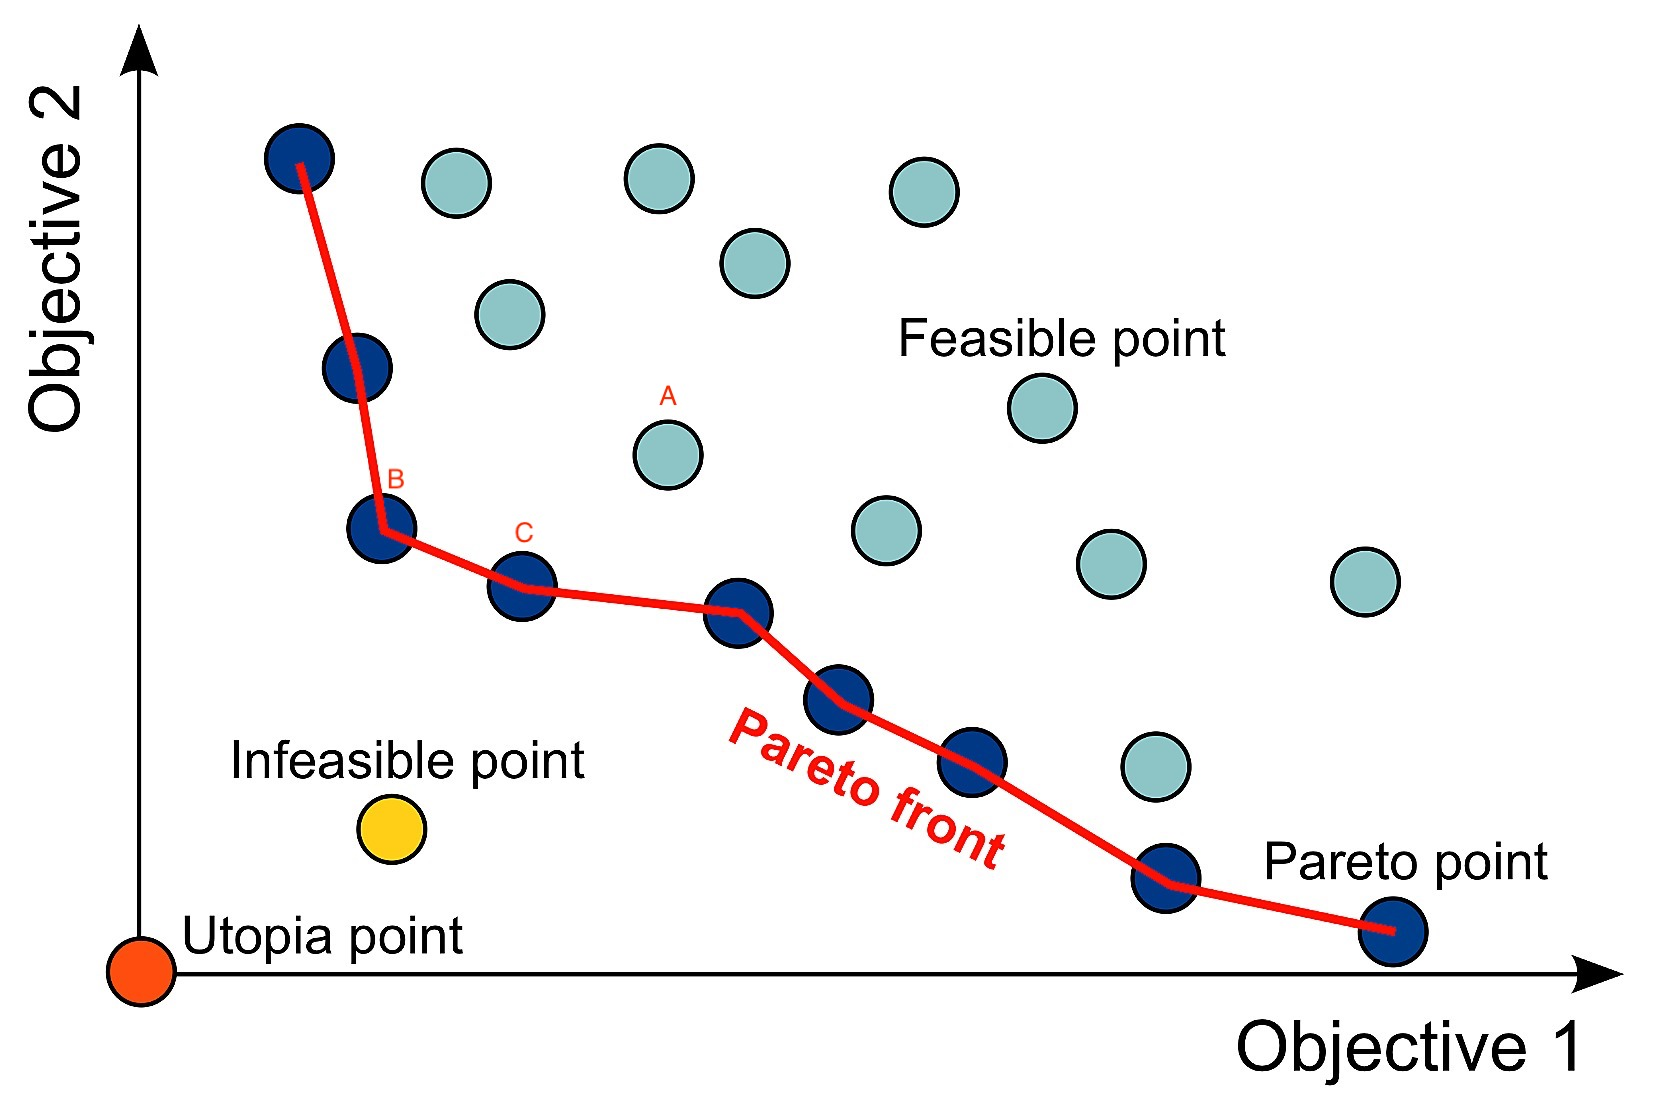
\includegraphics[width=0.66\linewidth]{img/pareto_front.JPG}
  \caption{\label{fig:paretofront}Pareto Front}
\end{figure}

Evolutionary algorithm such as the \emph{NSGA-II}\footnote{\url{https://ieeexplore.ieee.org/document/996017}} is a standard approach in solving multi-objective optimization problem. The algorithm is similar to a classical evolutionary algorithm. However the selection mechanism is different. The algorithm applies a pareto-based ranking scheme. This means that a rank is assigned to each individual based on nondominance - individuals that are not dominated by another get highest rank. Similarly as in EA, parents produce a new offspring population using genetic operators (i.e. crossover and mutation).

\begin{figure}[H]
  \centering
  \begin{subfigure}[t]{0.55\textwidth}
    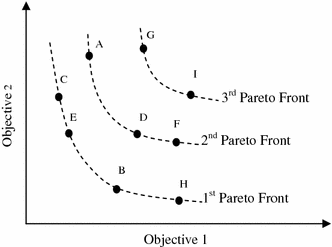
\includegraphics[width=\textwidth]{img/pareto_fronts.PNG}
    \caption{\label{fig:fronts}Pareto Fronts}
  \end{subfigure}
  \hfill
  \begin{subfigure}[t]{0.43\textwidth}
    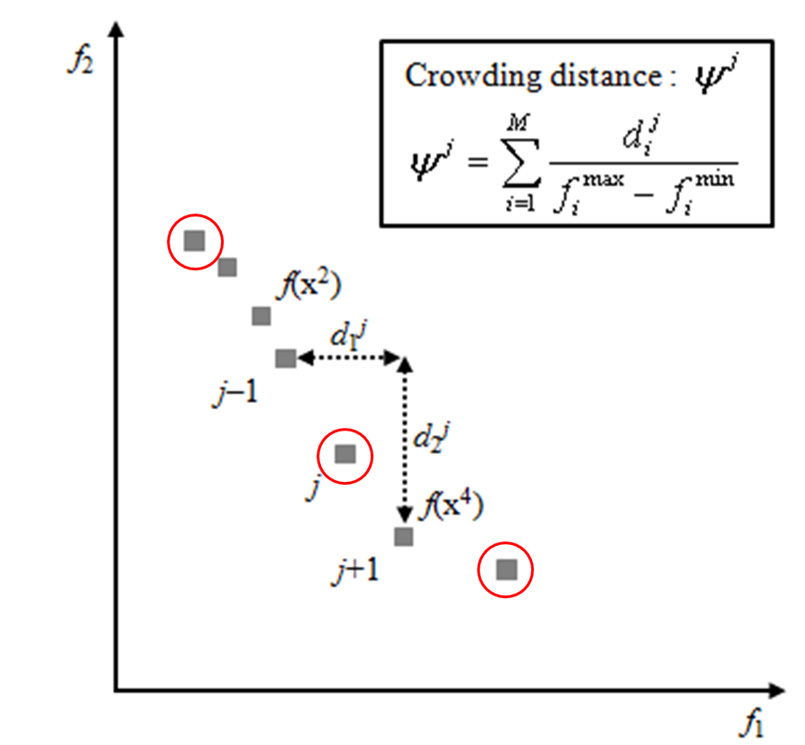
\includegraphics[width=\textwidth]{img/crowding_distance.JPEG}
    \caption{\label{fig:endings}Crowding Distance}
  \end{subfigure}
  \caption{\textit{Pareto Fronts} and \textit{Crowding Distance}.}
  \label{fig:action-ending-diagram}
\end{figure}


Parents and offsprings are combined together and are sorted into different fronts, determined by their ranking. Then a secondary sorting strategy is applied by calculating the crowding distance for each individual within their fronts. The best individuals are either in the lower fronts (assuming that the objective values are to be minimized) or in the same front with higher crowding distance. The crowding distance is calculated as the sum of the cubic distance of the objective values between the neighbouring solutions of the individual. This ensures to maintain diversity and spread of solutions - crowded solutions areas are less preferred than sparsely crowded solutions in the solution area. Next generation is created by copying the best solutions (\emph{elitism}) or the fist N individuals from the population of parents and offsprings. A more detailed flow diagram of the sorting procedure is depicted in the following figure \ref{fig:nsga}.

\begin{figure}[H]
  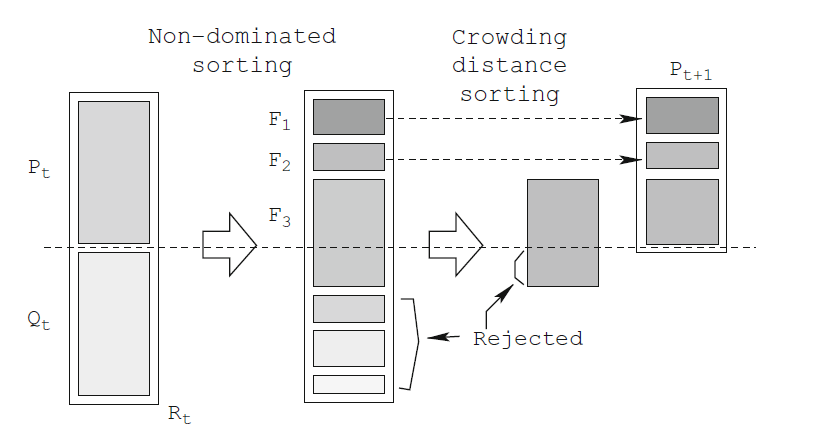
\includegraphics[width=0.66\linewidth]{img/nsga.PNG}
  \caption{\label{fig:nsga}Sorting procedure in NSGA-II}
\end{figure}

The implementation of the NSGA-II algorithm is provided by DEAP\footnote{\url{https://deap.readthedocs.io/en/master/}} evolutionary computation framework.

\subsection{NEAT}

NeuroEvolution of Augmenting Topologies \footnote{\url{http://nn.cs.utexas.edu/downloads/papers/stanley.ec02.pdf}} is a genetic algorithm for evolving both weights and topology of artificial neural networks. NEAT starts with minimal ANN structure and grows incrementally, which ensures low dimensionality of the connection weights and therefore minimizes the search space. The main traits of NEAT are \emph{genetic encoding, competing convention, speciation}.

NEAT encode networks with direct encoding schemes. The genome contains a list of \emph{connection genes} and list of \emph{nodes genes} which appears in the phenotype. Node genes represents inputs, hidden nodes, and outputs that can be connected. Whether a in-node and out-node is connected is expressed in the \emph{connection gene}. Additionally each connection gene contains a \emph{innovation} number. A genetic encoding of an individual can bee seen in figure \ref{fig:genome}.

\begin{figure}[H]
  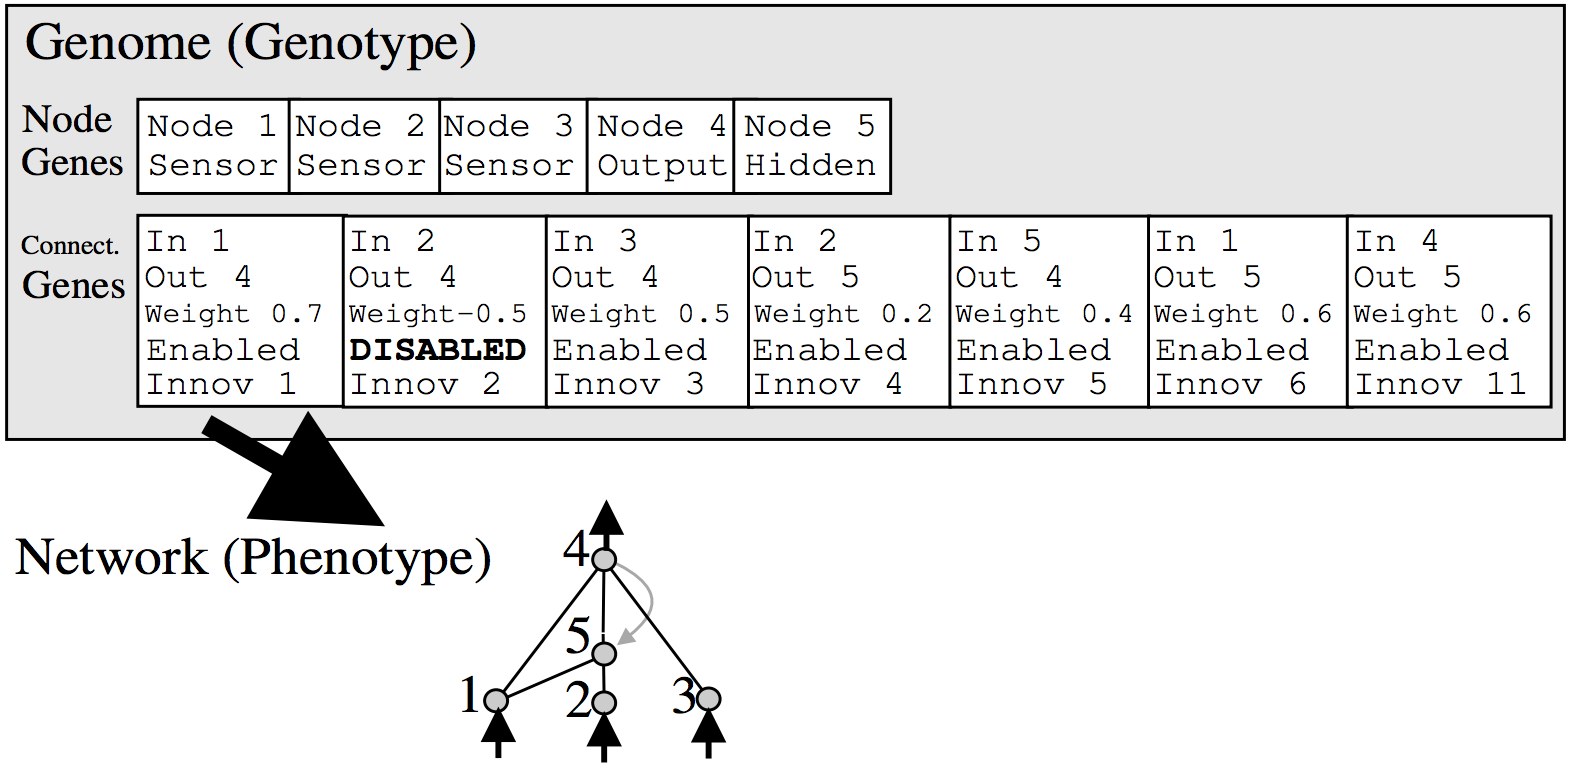
\includegraphics[width=0.66\linewidth]{img/neat_encoding.PNG}
  \caption{\label{fig:genome}Genetic encoding of individual}
\end{figure}

Mutation in NEAT can occur in three different ways. Connections weights are mutated just like in any neuroevolution, the value of the connection gene is mutated. Structural mutations are \emph{add connection and add node}. In \emph{add connection} mutation, a new connection gene is added with random weight connecting two previously unconnected nodes. Adding a new node, consists of splitting the existing connection between two nodes. The new node is added between these two previously connected nodes. The new connection leading to the new node receives the weight of 1, and the new connection leading out from the new node receives the old connection weight that was previously connecting the two nodes. The new connection of weight 1 minimize the initial affect of the mutation, this ensures that the network have time to optimize, because of \emph{speciation}. An example of this mutation can bee seen in figure\ref{fig:add_node}.

\begin{figure}[H]
  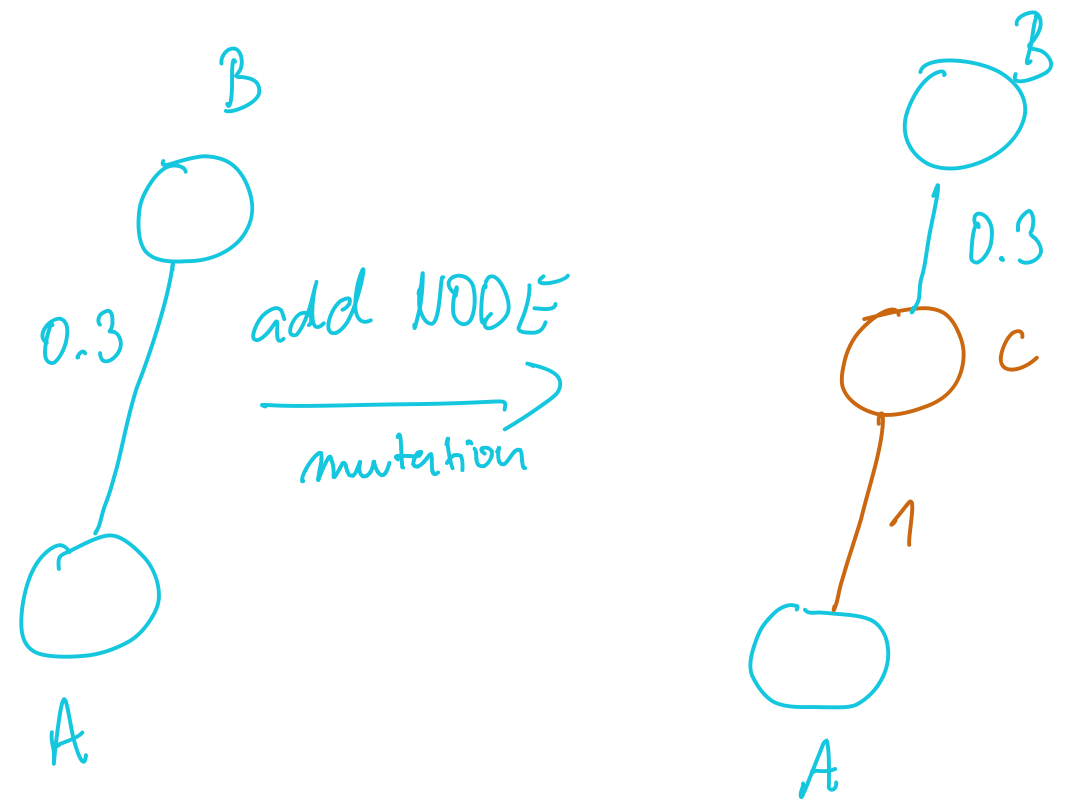
\includegraphics[width=0.56\linewidth]{img/add_node.JPEG}
  \caption{\label{fig:add_node}\emph{Add node} mutation operator in NEAT}
\end{figure}

\emph{Competing convention} is when individuals can express a solution to the same problem with different encoding. An example is depicted in figure \ref{fig:competing_convention}. The two networks compute the same function, even though their genetic encoding is different (hidden units appears in different order). This make crossover difficult, by one-point recombination of parents, both children lost crucial genetic information of their parents.

\begin{figure}[H]
  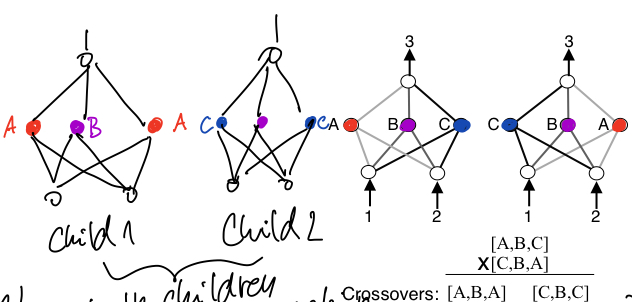
\includegraphics[width=0.56\linewidth]{img/competing_convention.JPEG}
  \caption{\label{fig:competing_convention}Competing Convention Problem}
\end{figure}

\emph{NEAT} is addressing this issues by \emph{global innovation number}, which enables genes to match up with genes of any individual in the population. More precisely, two genes with the same innovation number represents the same structure, because they are both derived from the same ancestral gene. Innovation numbers are unique and never change. Whenever two genomes mate, their offspring inherits the same innovation numbers on each gene.

When crossover is applied, the genomes are lined up with respect to the innovation number, see figure \ref{fig:crossover}. Genes that matches innovation number of both parents are called \emph{matching} gene. Genes that are not matched are called either \emph{disjoint} or \emph{excess}. During mating, \emph{matching} genes are randomly choose from either matching parent, whereas all \emph{disjoint} and \emph{excess} are included from the more fit parent.

\begin{figure}[H]
  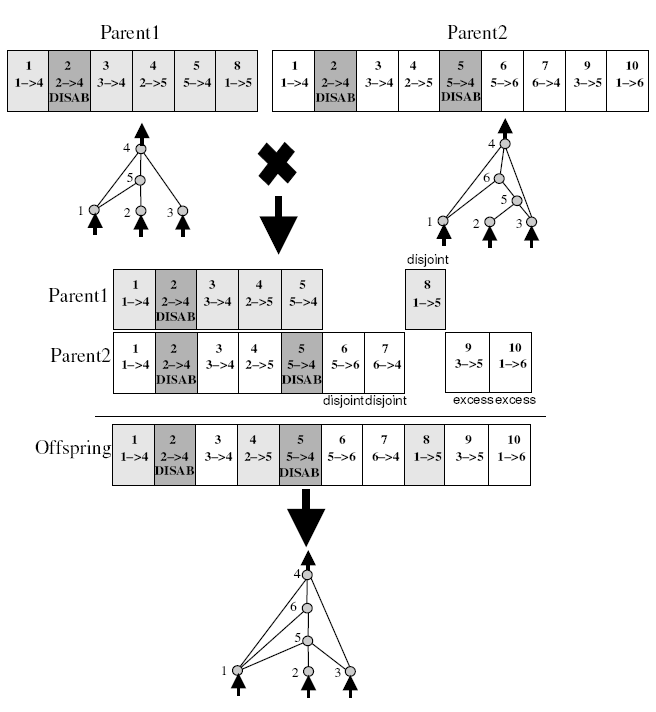
\includegraphics[width=0.5\linewidth]{img/crossover.PNG}
  \caption{\label{fig:crossover}Matching genomes innovation numbers}
\end{figure}


\emph{Speciations} in NEAT allows to divide the population into species according to topological similarities. Speciations ensures that topological innovations are protected and they have time to optimize their structure by competing within their niche. The implementation of speciation is exploited by measuring the compatibility distance according to the number of \emph{disjoint} and \emph{excess} genes between genomes. An ordered list of species is maintained. Species are represented by a random genome inside the species from previous generations. Each generation and individual is placed into the species in which the representative individual of that species is compatible with the current individual. If the individual is incompatible within any existing species, a new species is created with the individual as its representative. 


\subsection{HyperNEAT}

Donec euismod iaculis pretium. Donec non massa elit. Phasellus sagittis magna et maximus dictum. Duis quis ullamcorper orci. Mauris interdum, elit eu tincidunt tempor, lectus mi venenatis purus, quis posuere tellus ex in magna. Phasellus tincidunt nibh eu tortor semper, et varius justo vulputate. Nullam dictum congue lacinia. Maecenas sagittis nulla quis leo fringilla viverra. Proin eget egestas nisl. Class aptent taciti sociosqu ad litora torquent per conubia nostra, per inceptos himenaeos. Pellentesque habitant morbi tristique senectus et netus et malesuada fames ac turpis egestas. Vestibulum a interdum tellus, a hendrerit ligula. Duis ut risus ut lacus maximus euismod. Integer quis justo sit amet sapien accumsan rutrum nec nec dolor. Aliquam laoreet scelerisque ante, quis hendrerit ipsum viverra tempor.

\subsection{Multi-Spatial Substrates}

Donec euismod iaculis pretium. Donec non massa elit. Phasellus sagittis magna et maximus dictum. Duis quis ullamcorper orci. Mauris interdum, elit eu tincidunt tempor, lectus mi venenatis purus, quis posuere tellus ex in magna. Phasellus tincidunt nibh eu tortor semper, et varius justo vulputate. Nullam dictum congue lacinia. Maecenas sagittis nulla quis leo fringilla viverra. Proin eget egestas nisl. Class aptent taciti sociosqu ad litora torquent per conubia nostra, per inceptos himenaeos. Pellentesque habitant morbi tristique senectus et netus et malesuada fames ac turpis egestas. Vestibulum a interdum tellus, a hendrerit ligula. Duis ut risus ut lacus maximus euismod. Integer quis justo sit amet sapien accumsan rutrum nec nec dolor. Aliquam laoreet scelerisque ante, quis hendrerit ipsum viverra tempor.

\section{Aseba and Thymio}

\emph{Thymio}\footnote{\url{https://www.thymio.org/home-en:home}} is a small robot produced by Mobsya\footnote{\url{http://www.mobsya.org/}} for educational purposes. It has 5 proximity sensors in front, 2 proximity sensors on the back as well as 2 grounds sensors. Thymio is also equipped with temperature sensor, various buttons for interaction, visual sensors etc. Detailed overview of all the components can bee seen in figure\ref{fig:thymio}. For this experiments purposes we use the new \emph{Wireless Thymio}, which enables us to control the robot with wireless dongle.

\begin{figure}[H]
  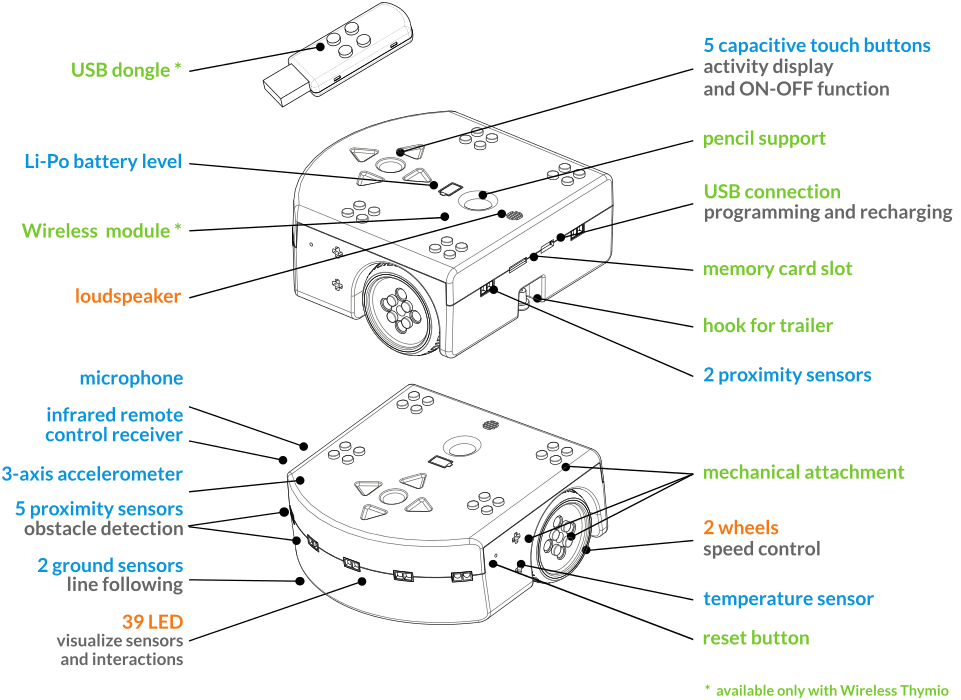
\includegraphics[width=0.6\linewidth]{img/thymio.PNG}
  \caption{\label{fig:thymio}Components of Thymio}
\end{figure}

Thymio can be programmed with \emph{Aseba}\footnote{\url{https://aseba.readthedocs.io/en/latest/about.html}}, which is set of tools that enables to program the robot within several programming environments, namely \emph{Visual, Blockly, Text, Scratch} programming. Aseba is shipped with a command-line utility tool called \emph{asebamedulla}, that allows to access an Aseba network through \emph{D-BUS}\footnote{\url{https://www.freedesktop.org/wiki/Software/dbus/}}. This enables to program Aseba-enabled devices, the Thymio robot, using third party languages, in our case Python. The \emph{Aseba Community Repository}\footnote{\url{https://github.com/aseba-community/aseba}} contains several examples how to interface with asebamedulla using D-Bus. Since our preferred language is Python, the python CLI\footnote{\url{https://github.com/aseba-community/aseba/blob/master/examples/clients/python-dbus/aseba.py}} was chosen, which is a thin wrapper around asebamedulla dbus interface. 

D-Bus is the main IPC system used in Linux: processes expose objects with a declared interfaces whose methods can be called from other processes. This is implemented by sending messages over D-Bus itself. The Aseba environment provides a D-Bus interface via the asebamedulla utility, which is in charge of transmitting to the robot hardware. The abstraction is in the form of a network of Thymio robots and processes listening on D-Bus, the so-called \emph{AsebaNetwork}. 

The goal of the Aseba D-Bus integration is not to be an alternative to any of the Aseba languages used to program the robots locally. Indeed, it is meant to provide integration with another system, on which not only the D-Bus deamon and asebamedulla are running, but also the programs utilizing the D-Bus interface, which are never transferred in any manner to the Thymio hardware. This in turn means that the robots are supposed to be continuously connected to the machine on which the Python script, in our case, is running.

The API consists ultimately in the interfaces that asebamedulla provides over D-Bus. Through this interface, we can retrieve information about the network, read and write variables, or send events.

\begin{lstlisting}[caption={\ The API that asebamedulla provides over D-Bus},language=Python,captionpos=b,label={Asebamedulla API},basicstyle=\small]
interface ch.epfl.mobots.EventFilter {
    method Void ListenEvent(UInt16 eventId)
    method Void ListenEventName(String eventName)
    method Void IgnoreEvent(UInt16 eventId)
    method Void IgnoreEventName(String eventName)
    signal Event(UInt16 id, String name, Array<SInt16> payloadData)
}

interface ch.epfl.mobots.AsebaNetwork {
    method Void LoadScripts(String fileName)
    method Array<String> GetNodesList()
    method Array<String> GetVariablesList(String nodeName)
    method Void SetVariable(String nodeName, String variableName, Array<SInt16> variableData)
    method Array<SInt16> GetVariable(String nodeName, String variableName)
    method Void SendEvent(UInt16 eventId, Array<SInt16> payloadData)
    method Void SendEventName(String eventName, Array<SInt16> payloadData)
    method ObjectPath CreateEventFilter()
}
\end{lstlisting}


The \emph{AsebaNetwork} interface allows to work with all of the nodes (robots) in the same network. There are methods to retrieve a list of the connected nodes ( \emph{GetNodesList} ) and to broadcast a global event, like \emph{SendEvent}. Global events are events that aseba nodes exchange within the aseba network. On the other hand, events that are internal to the node are called \emph{local events}. \emph{SetVariable} and \emph{GetVariable}, which write and read respectively native variables of the Aseba scripting language.

Asebamedulla expose the interface \emph{EventFilter} which allows to manage events. An application that wants to listen to events have register events with \emph{ListenEventName} or \emph{ListenEvent} be notified when an event occurs. The application can receive these events through the \emph{Event} signal, these events correspond to the global events of the Aseba language.

\section{Robotic Simulator}

Donec euismod iaculis pretium. Donec non massa elit. Phasellus sagittis magna et maximus dictum. Duis quis ullamcorper orci. Mauris interdum, elit eu tincidunt tempor, lectus mi venenatis purus, quis posuere tellus ex in magna. Phasellus tincidunt nibh eu tortor semper, et varius justo vulputate. Nullam dictum congue lacinia. Maecenas sagittis nulla quis leo fringilla viverra. Proin eget egestas nisl. Class aptent taciti sociosqu ad litora torquent per conubia nostra, per inceptos himenaeos. Pellentesque habitant morbi tristique senectus et netus et malesuada fames ac turpis egestas. Vestibulum a interdum tellus, a hendrerit ligula. Duis ut risus ut lacus maximus euismod. Integer quis justo sit amet sapien accumsan rutrum nec nec dolor. Aliquam laoreet scelerisque ante, quis hendrerit ipsum viverra tempor.

\section{Experiments}

Donec euismod iaculis pretium. Donec non massa elit. Phasellus sagittis magna et maximus dictum. Duis quis ullamcorper orci. Mauris interdum, elit eu tincidunt tempor, lectus mi venenatis purus, quis posuere tellus ex in magna. Phasellus tincidunt nibh eu tortor semper, et varius justo vulputate. Nullam dictum congue lacinia. Maecenas sagittis nulla quis leo fringilla viverra. Proin eget egestas nisl. Class aptent taciti sociosqu ad litora torquent per conubia nostra, per inceptos himenaeos. Pellentesque habitant morbi tristique senectus et netus et malesuada fames ac turpis egestas. Vestibulum a interdum tellus, a hendrerit ligula. Duis ut risus ut lacus maximus euismod. Integer quis justo sit amet sapien accumsan rutrum nec nec dolor. Aliquam laoreet scelerisque ante, quis hendrerit ipsum viverra tempor.

\section{Mixed Reality}

Donec euismod iaculis pretium. Donec non massa elit. Phasellus sagittis magna et maximus dictum. Duis quis ullamcorper orci. Mauris interdum, elit eu tincidunt tempor, lectus mi venenatis purus, quis posuere tellus ex in magna. Phasellus tincidunt nibh eu tortor semper, et varius justo vulputate. Nullam dictum congue lacinia. Maecenas sagittis nulla quis leo fringilla viverra. Proin eget egestas nisl. Class aptent taciti sociosqu ad litora torquent per conubia nostra, per inceptos himenaeos. Pellentesque habitant morbi tristique senectus et netus et malesuada fames ac turpis egestas. Vestibulum a interdum tellus, a hendrerit ligula. Duis ut risus ut lacus maximus euismod. Integer quis justo sit amet sapien accumsan rutrum nec nec dolor. Aliquam laoreet scelerisque ante, quis hendrerit ipsum viverra tempor.

\section{Summary}

Donec euismod iaculis pretium. Donec non massa elit. Phasellus sagittis magna et maximus dictum. Duis quis ullamcorper orci. Mauris interdum, elit eu tincidunt tempor, lectus mi venenatis purus, quis posuere tellus ex in magna. Phasellus tincidunt nibh eu tortor semper, et varius justo vulputate. Nullam dictum congue lacinia. Maecenas sagittis nulla quis leo fringilla viverra. Proin eget egestas nisl. Class aptent taciti sociosqu ad litora torquent per conubia nostra, per inceptos himenaeos. Pellentesque habitant morbi tristique senectus et netus et malesuada fames ac turpis egestas. Vestibulum a interdum tellus, a hendrerit ligula. Duis ut risus ut lacus maximus euismod. Integer quis justo sit amet sapien accumsan rutrum nec nec dolor. Aliquam laoreet scelerisque ante, quis hendrerit ipsum viverra tempor.


\end{document}
